\textbf{\subsection{Расчет регулятора усиления}}

  Регулятор усиления обычно ставится после первого или второго каскада предварительного усиления. В качестве регулятора могут быть использованы нагрузочные сопротивления каскадов, например сопротивление в цепи эмиттера эмиттерного   повторителя.
  \par
     $R_{\text{ВЫХ.ПРЕД}} = 5 $кОм  и   $R_{\text{ВХ.СЛЕД}} = 88.5 $кОм  
  \begin{equation}
   \label{eq:equation6_22}
     R_{\text{У}}=\sqrt{R_{\text{вых.пред}}\cdot {R_{\text{вх.след}}}}=\sqrt{R_{\text{Г}}\cdot R_{\text{кпу}}}=\sqrt{8850 \cdot 5000}=21~\text{кОм}
   \end{equation}

   \begin{figure}[htbp]
    \center{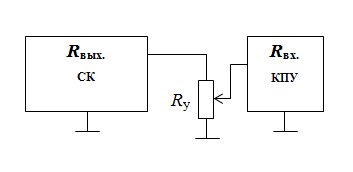
\includegraphics[width=0.4\linewidth]{picture_6}}
    \caption{Схема регулятора усиления}
    \label{figure:p3_1}
  \end{figure}
     

     